\begin{abcliste}
\abc Bei \tCO\ liest man ab: $v_\mathrm{A} = \vAO$ und
\begin{align}
 v_\mathrm{B} &= \vBtF = \frac{\vB}{\tB}\cdot\tC = \vBt \approx \vBtP{0}{2}
\end{align}
$\result{\text{B ist schneller}}$: Der Graph von B liegt bei \tCO\ höher.

\abc Wie weit ein Fahrzeug gefahren ist, zeigt nicht die Höhe des Graphen, sondern die Fläche darunter von $0$ bis \tCO:
\begin{center}
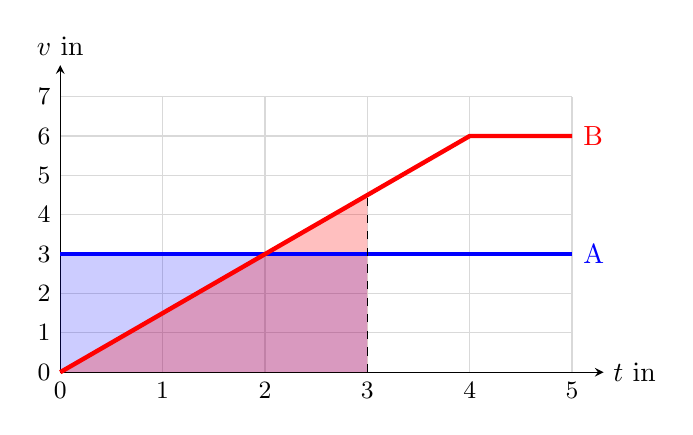
\begin{tikzpicture}[>=stealth, x=1.3cm, y=0.5cm]
 \draw[gray!30] (0,0) grid[xstep=1, ystep=1] (5,7);
 \draw[->] (0,0) -- (5.308,0) node[right] {$t$ in \si{\second}};
 \draw[->] (0,0) -- (0,7.8) node[above] {$v$ in \si{\meter\per\second}};
 \foreach \tk in {0,1,2,3,4,5} \node[below] at (\tk,0) {\small $\tk$};
 \foreach \yk in {0,1,2,3,4,5,6,7} \node[left] at (0,\yk) {\small $\yk$};

 \fill[blue, opacity=0.2] (0,0) rectangle (3,3);
 \fill[red, opacity=0.25] (0,0) -- (3,4.5) -- (3,0) -- cycle;
 \draw[ultra thick, blue] (0,3) -- (5,3) node[right] {A};
 \draw[ultra thick, red] (0,0) -- (4,6) -- (5,6) node[right] {B};
 \draw[dashed] (3,0) -- (3,4.5);
\end{tikzpicture}
\end{center}
\begin{align}
 s_\mathrm{A} &= \sAF = \vA\cdot\tC = \sA \approx \result{\sAP{0}{2}} \\
 s_\mathrm{B} &= \sBF = \frac{1}{2}\cdot\aB\cdot\left(\tC\right)^2 = \sB \approx \result{\sBP{0}{3}}
\end{align}
$\result{\text{A ist weiter vorne}}$, obwohl B in diesem Moment schneller ist. Bis \SI{2}{\second} war B langsamer als A; diesen Rückstand hat B bis \tCO\ noch nicht aufgeholt.

\abc B holt A ein, wenn die beiden Flächen gleich gross sind:
\begin{align}
 v_\mathrm{A}\,t_\mathrm{M} &= \frac{1}{2}\,a_\mathrm{B}\,t_\mathrm{M}^2 \quad\Rightarrow\quad t_\mathrm{M} = \tMF = \frac{2\cdot\vA}{\aB} = \tM \approx \result{\tMP{0}{1}}
\end{align}
Das ist genau der Zeitpunkt, bei dem B seine Endgeschwindigkeit erreicht. Beide sind dann \sMP{0}{2} gefahren.
\end{abcliste}
